\documentclass[../../main]{subfiles}

\begin{document}
\chapter{数ベクトル空間}
\label{chapter:numerical_vector_space}

\begin{lead}
  \cref{chapter:numerical_vector_space}で書く予定のことを並べておく.
\end{lead}

\section{直交射影}
\subsection{直交射影}
\begin{figure}[htbp]
  \centering
  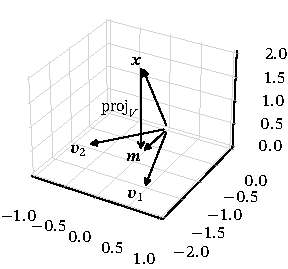
\includegraphics{projection.pdf}
\end{figure}

\subsection{直交補空間}
\begin{figure}[htbp]
  \centering
  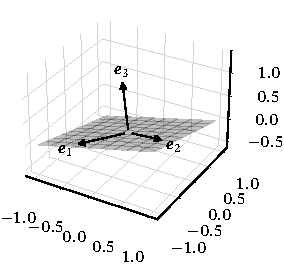
\includegraphics{orthogonal_complement.pdf}
\end{figure}
\subsection{スペクトル定理}

\section{最小二乗問題}
\subsection{最小二乗問題}
\subsection{特異値分解}
\subsection{擬似逆行列}

\section{離散フーリエ変換}

\section{多重解像度解析}

\begin{subappendices}
\section{主成分分析}
\begin{figure}[htbp]
  \begin{minipage}{\linewidth/2}
    \centering
    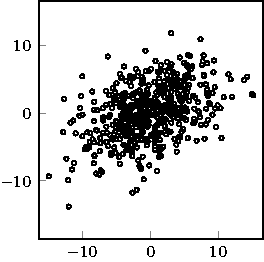
\includegraphics{scatter.pdf}
  \end{minipage}%
  \begin{minipage}{\linewidth/2}
    \centering
    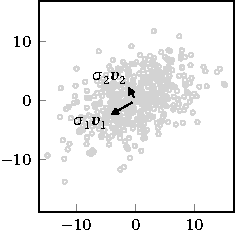
\includegraphics{pca.pdf}
  \end{minipage}
\end{figure}

\section{低ランク近似}
\section{窓関数}
\end{subappendices}

\section*{演習問題}
\addcontentsline{toc}{section}{演習問題}

\end{document}
